%*******************************************************************************
%*********************************** Chapter XXXXXXXX *****************************
%*******************************************************************************

\chapter{The 35 ton camera system} \label{chap:Cameras} %Title of chapter

\nomenclature[z-HV]{HV}{High Voltage}
\nomenclature[z-CMOS]{CMOS}{Complementary Metal-Oxide Semiconductor}
\nomenclature[z-CCD]{CCD}{Charge-Couple Device}
\nomenclature[z-DVR]{DVR}{Digital Video Recorder}


\graphicspath{{The35tonCameras/Figs/Raster/}{The35tonCameras/Figs/PDF/}{The35tonCameras/Figs/Vector/}}

As noted in Section~\ref{sec:The35tonDetector}, a camera system which was designed and built by the University of Sheffield, was installed in Run II of the 35 ton prototype. The reason for this was to monitor the cryostat for any potential high voltage (HV) breakdowns. The occurrence of a HV breakdown in liquid Argon (LAr) is possible due to the large electric fields which are required for experiments such as DUNE. For example, when the drift field of 500 V cm$^{-1}$ will be applied to the DUNE far detector (FD), it will require a bias voltage of -180 kV~\citep{DUNECDR_V4} on the cathode plane. As the breakdown field has recently been measured to be much lower than this, at around 40 kV cm$^{-1}$~\citep{BlatterEField}, some form of monitoring is required. \\

To this end, a Complementary Metal-Oxide Semiconductor (CMOS) camera is used within the LAr to observe any potential HV breakdowns in the 35 ton cryostat. Charge-Coupled Device (CCD), and CMOS cameras have previously been used to do this. This has never been done before using cameras which are immersed in LAr. Previously, cameras have either used viewing ports which were built into the detector, or were inside enclosures which had a raised temperature~\citep{BlatterEField,BERNcam,LAPD,Liverpool,Weizmannbubbles}. As well as looking for HV breakdowns, the cameras also visually monitored the TPC and cryogenic components as filling occurred. The information contained in this section is a summary of the paper detailing the performance of the cameras in the 35 ton prototype~\citep{CameraPaper}. The author was responsible for the fabrication of, initial setup, and maintainence of all equipment which was used at Fermilab, including ensuring that the camera system met all safety standards. The author was not responsible for the studies which were performed to select the cameras used, or in the design and construction of the camera mounting modules. \\

%********************************** %Second Section  *************************************
\section{The selection and characterisation of cameras} \label{sec:CamSelec} %Section - X.2
As the cameras in the 35 ton are submerged in LAr, they are required to work at cryogenic temperatures. The cameras are also required to be sensitive enough to visible light, that they can observe the sparks created by the HV breakdowns, this means that the cameras must have low thermal noise. CMOS cameras are used as there are many cameras which are rated to work down to temperatures of -40 $^{\circ}$C. CMOS cameras are also found to have lower leakage currents, improved mobility, and lower thermal noise, at temperatures around 100K~\citep{thermalnoise1,thermalnoise2}. \\

When a shock test, consisting of submersion in LAr, is performed on a range of CMOS cameras, it is found that the most reliable camera is a \emph{Floureon} car reversing camera. It is believed that the simplicity of this camera allows it to be relatively unaffected when operating at low temperatures. This is because it has a simple internal circuit consisting of resistors, capacitors, a crystal oscillator, and a flash memory chip. \\

It is important to determine the effect which operation at cryogenic temperatures has on the performance of the cameras. To do this, the frame rate, and resolutions in both time and space, whilst submerged in LAr, are compared with a complementary set of measurements made at room temperature in air. It is found that the frame rate, and resolution in time, are both unaffected at 50 Hz, and 20 ns, respectively. The timing resolution of the cameras was determined using LED's in a dark box, which were connected to a pulse generator that generated pulses of variable widths. It was found that in both air and LAr, the cameras were able to trigger on pulses once they were longer than 20 ns. The spatial resolution, which was also found to be unaffected within systematic errors, was measured by varying the distance between two optical fibres, connected to a single LED, until the light from both optical fibres could no longer be resolved. \\

When attempting to use the cameras to locate HV breakdowns, it is necessary to develop a triggering mechanism. The camera signals are read out using a digital video recorder (DVR), which is remotely accessible using SwannView Link, a commercially available surveillance program. The SwannView Link software detects movement between successive frames, and so in normal use will begin recording if, for example, a person enters the field of view. The length of time for which a video is recorded, and the number of frames which are recorded before the trigger, can be configured by the user. The monitoring for HV breakdowns is remarkably similar to this application, as when a breakdown occurs the field of view would be illuminated by a large flash of light, which was not present in the previous frame. When determining if a breakdown has occurred, a threshold in the number of pixels which change between consecutive frames is used. It is also possible to select only a limited number of pixels, if for example, some regions of the cameras field of view are rapidly changing, or if the expected change would only be in a very precise location. This was the case with some of the cameras in the 35 ton, where there was elevated thermal noise in some regions of the camera pictures. \\

The ability of the cameras to measure HV breakdowns, using the above triggering system, was tested prior to installation in the 35 ton. In the tests, a high voltage was applied across a printed circuit board, until breakdown was observed. When breakdowns occurred, the triggers which the cameras recorded showed sparks which were highly localised and lasted over multiple frames. \\

%********************************** %Second Section  *************************************
\section{The design of the camera system} \label{sec:CamDesign} %Section - X.2

As will be noted at the start of Chapter~\ref{chap:35tonData}, the 35 ton detector was filled with LAr for over 3 months, and so the shock tests performed with liquid nitrogen were not sufficient to guarantee continuous running of the cameras during the entire 35 ton run. It is also necessary to protect against the prospect of a power failure, which could cause the cameras to be turned off for a large period of time. Should this occur, the cameras would have to be able to be turned on at cryogenic temperatures. During testing, it was found that whilst some of the \emph{Floureon} cameras were able to do this, this was not the case for all cameras. Only cameras which were found to be able to be turned off and on again in the cold were used in the 35 ton. The process of turning a camera off and on again is referred to here as a camera being ``power cycled.'' \\

As the failure rate of the cameras was non-zero, and because the 35 ton run was scheduled to be much longer than any cameras had been tested in the cold, it was decided that it was prudent to build a self-contained module to house the cameras. A heater, consisting of two resistors placed either side of the camera, was installed inside the camera module. This is because it was found that some of the cameras which failed the shock tests, could be power cycled when they were exposed to an elevated, though still cryogenic, temperature. A temperature sensor was also placed in the modules, so that the increase in temperature during normal operation, and also during heating, could be measured. It was found that the cameras caused the internal temperature of the module to rise by roughly 15 K, though the temperature of the glass viewing panel, and the external camera module, were unchanged. It was also found that with the heater operational, the internal temperature of the module could rise by as much as 80 K after 17 minutes. During operation, the heaters and power supply to the cameras were controlled using a custom-built, remotely controllable device, built by Bob Bridgeland, at the University of Warwick. The temperature from the PT100 sensor was processed by another custom-made device, the output of which was read into a computer, using a NI USB-6009 device. \\

A schematic of a camera module is shown in Figure~\ref{fig:CamSchem}. Figure~\ref{fig:CamModule} shows a picture of a sealed camera module, with the individual components inside a module next to it. \\

\begin{figure}
  \centering
  \begin{subfigure}{0.45\textwidth}
    \centering
    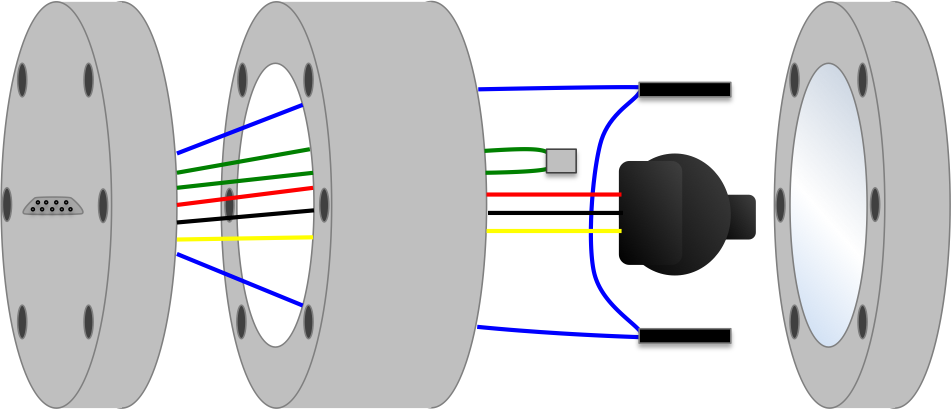
\includegraphics[width=\textwidth]{cam_in_housing_diagram}
    \caption{A schematic of the camera module.}
    \label{fig:CamSchem}
  \end{subfigure}
  \hspace{0.08\textwidth}
  \begin{subfigure}{0.45\textwidth}
    \centering
    \includegraphics[width=\textwidth]{camera_module_explode_labels}
    \caption{A sealed camera module, along with the components contained inside the module.}
    \label{fig:CamModule}
  \end{subfigure}
  \caption[The components which made up a camera module used in the 35 ton camera system]
          {The components which made up a camera module used in the 35 ton camera system. Left: a schematic representation of the components in the camera modules, with wires from the PT100 temperature sensor (green), the heating resistors (blue) and camera (red, blue, yellow), connected to a 9-pin D-sub feed through, shown on the left of the image. Right: the physical components, both inside and outside, a module. A camera, a heater and a temperature sensor, can all be seen. A PTFE holder is used to ensure that the components remain in the desired locations, with the camera pressed up to the glass viewing panel. Bolts are used to ensure that the camera modules are leak tight.}
\end{figure}

It was necessary to mount the camera modules inside the 35 ton. This was achieved using a custom-designed mounting bracket, an example of which is shown in Figure~\ref{fig:CamMount}. The mounts were fixed to existing cryogenic pipework, and could be freely rotated, so that the cameras could be pointed towards specific regions of interest. This meant that the camera mounts had two degrees of freedom, as well as being able to freely placed on the cryogenic pipes. \\

\begin{figure}
  \centering
  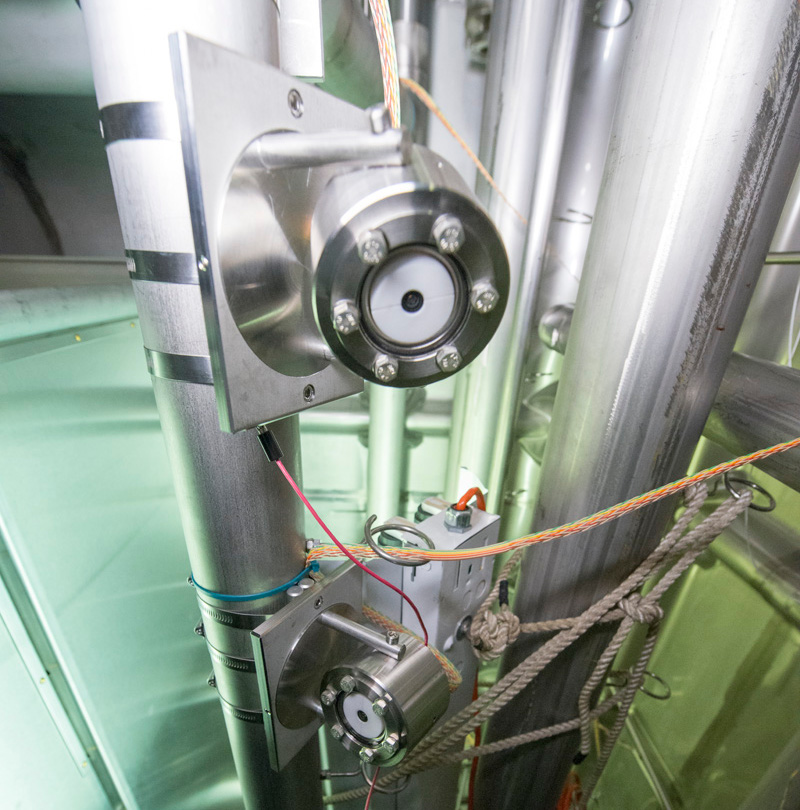
\includegraphics[width=0.45\textwidth]{cammount35tcrop}
  \caption[Two camera modules which are mounted in the 35 ton prototype detector]
          {Two camera modules which are mounted in the 35 ton prototype detector. The mounts are affixed to a 3'' SCH cryogenic pipe. The multi-coloured ribbon cables which were used to carry the camera signals outside of the cryostat can be seen in the picture.}
  \label{fig:CamMount}
\end{figure}

However, before the cameras could be installed in the 35 ton cryostat, several safety reviews had to be completed, in order to comply with safety standards set out by Fermilab, the host lab for the 35 ton prototype. These consisted of a review of the cable rack which was used during operations, plus individual reviews for the components which were custom-built. There was also a further review covering the camera system as a whole when it was operational. Only after the successful completion of all of these reviews was the camera system allowed to be installed, and ran unsupervised, inside the 35 ton cryostat. \\

In order to satisfy the safety requirements, adequate grounding of the rack, and all of its components, had to be displayed. This requirement extended to ensuring that the cables used in the system, which were assembled at Fermilab, would not introduce any potential ground loops into the 35 ton system. This meant that detailed diagrams of the individual components, and how they linked together to form the camera system, had to be produced. The detailed diagram which was produced representing the entire camera system is shown in Figure~\ref{fig:CamSysDiagram}. \\

\begin{figure}
  \centering
  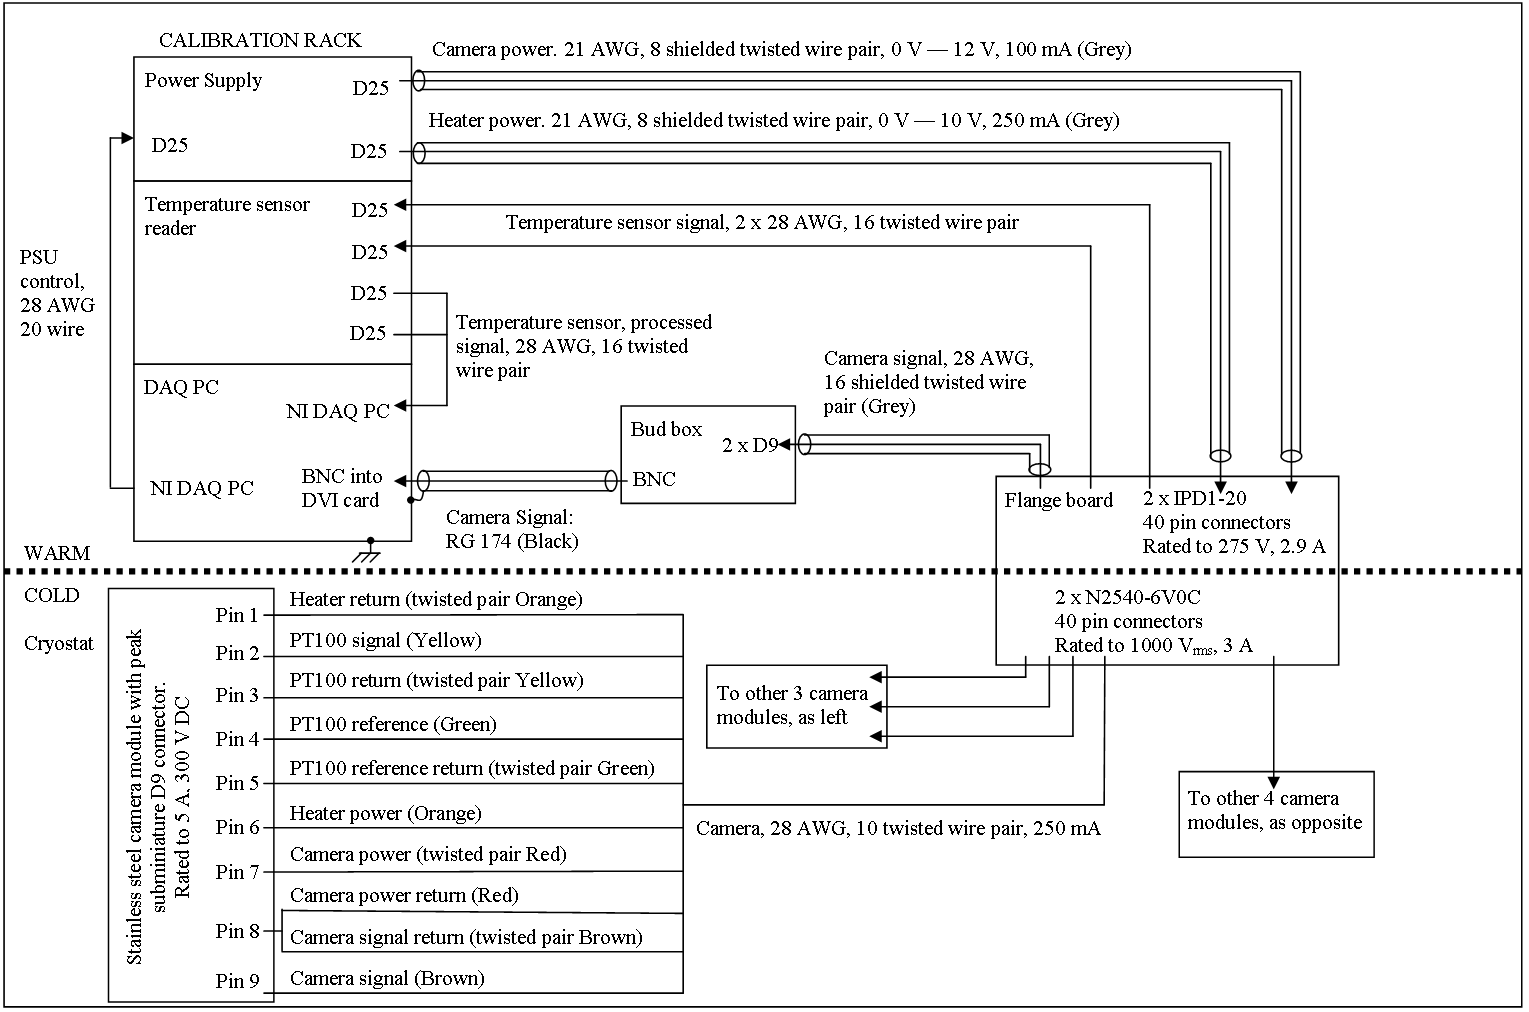
\includegraphics[width=0.95\textwidth]{Camera_Block_diagram}
  \caption[The system diagram for the 35 ton camera system]
          {The system diagram for the 35 ton camera system. The contents of the rack which was used in the camera system (top left), the wires which were terminated at the flange board (right), and the signals that each of the wires connected to the cameras carried (bottom left), are shown. In addition to this, the wire gauge (in units of American Wire Gauge), along with the voltages and currents which they carried, and the number of wires which were bound together, are shown for the connections between each subsystem and the flange board. Shielded wires are shown as wires with cylindrical covers around them, such as the wire labelled ``Camera power.'' In total there were eight camera modules installed in the cryostat, connected in two groups of four cameras, to the flange board by two 40 pin connectors.}
  \label{fig:CamSysDiagram}
\end{figure}

%********************************** % Fifth Section  *************************************
\section{Performance in the 35 ton}  %Section - X.5
In total eight cameras were installed inside the 35 ton cryostat, the locations of which were selected to maximise the potential of observing any HV breakdowns which may occur. It was decided that the cameras would be focused on the following parts of the detector;
\begin{itemize}
\item The top right hand corner of the cathode.
\item The bottom right hand corner of the cathode.
\item The top left hand corner of the cathode.
\item The bottom left hand corner of the cathode.
\item The location of the high voltage feedthrough.
\item The ullage - the gap between the top of the TPC, and the roof of the cryostat
\item The cool down sprayers - this was only for use during cool down, to check that they were operating as expected.
\item The phase separator - this was for use during operation to ensure that it was running as expected.
\end{itemize}
Upon installation in the cryostat, some calibration images were taken for each camera, these are shown in Figure~\ref{fig:CamFOV}. \\

\begin{figure}
 \centering
 \minipage{0.4\textwidth}
   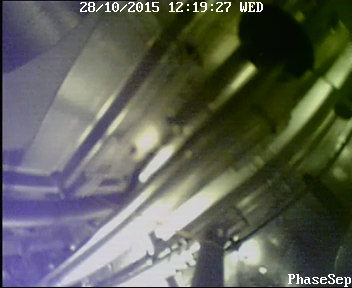
\includegraphics[width=\linewidth]{phasesep}
 \endminipage
 \minipage{0.4\textwidth}
  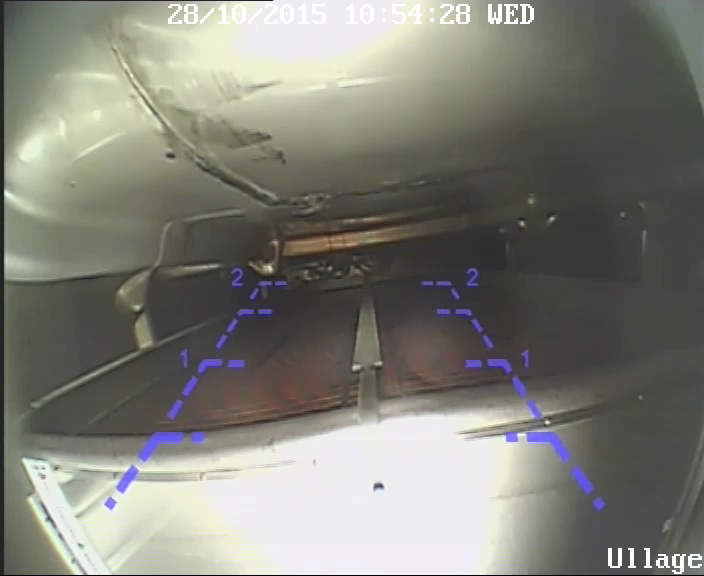
\includegraphics[width=\linewidth]{ullage}
 \endminipage

 \minipage{0.4\textwidth}
  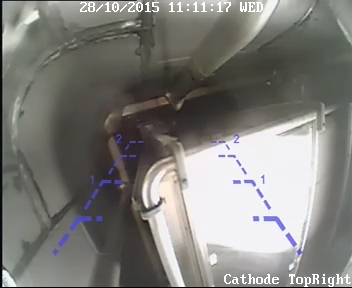
\includegraphics[width=\linewidth]{cathodetr}
 \endminipage
 \minipage{0.4\textwidth}
   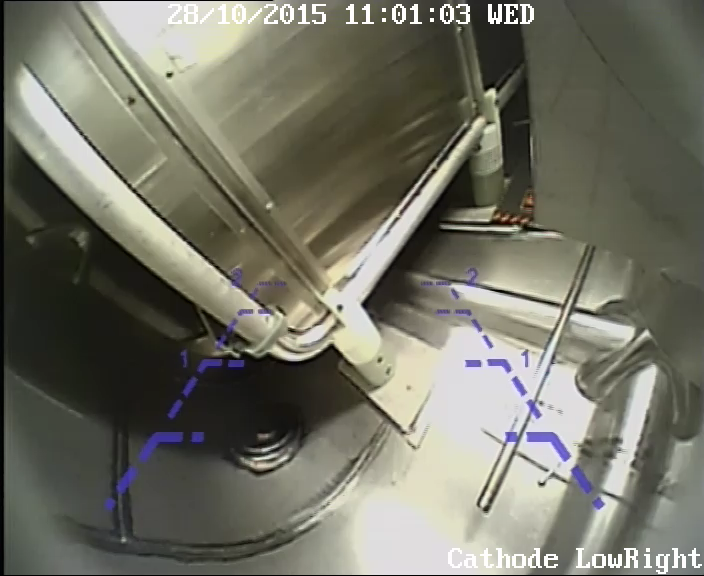
\includegraphics[width=\linewidth]{cathodelr}
 \endminipage

 \minipage{0.4\textwidth}
   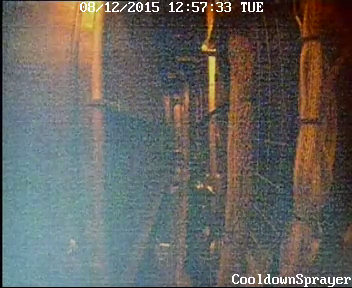
\includegraphics[width=\linewidth]{cooldownsp}
 \endminipage
 \minipage{0.4\textwidth}
   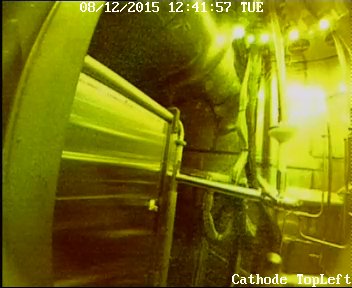
\includegraphics[width=\linewidth]{cathodetl}
 \endminipage

 \minipage{0.4\textwidth}
   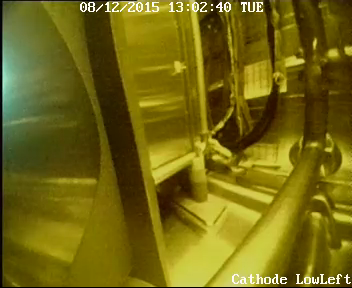
\includegraphics[width=\linewidth]{cathodell}
 \endminipage
 \minipage{0.4\textwidth}
   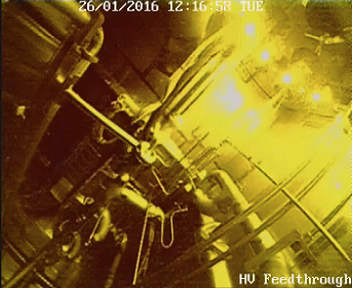
\includegraphics[width=\linewidth]{hvft}
 \endminipage
 \caption[The calibration images for the 8 cameras used in the 35 ton camera system]
         {The calibration images for the 8 cameras used in the 35 ton camera system.  The images from left to right, top to bottom, show the following: phase separator, ullage, cathode top right, cathode bottom right, cool down sprayers, cathode top left, cathode bottom left, and high voltage feed through.  The upper four images were taken with a halogen light illuminating the cryostat, prior to it being sealed up.  The lower four images were taken after the cryostat was sealed, and was illuminated by a ring of LEDs.  All images are left-right inverted due to software.}
 \label{fig:CamFOV}
\end{figure}

As previously mentioned, the cameras used were car reversing cameras, and so this is why there are distance lines on some of the images in Figure~\ref{fig:CamFOV}. From Figure~\ref{fig:CamFOV}, it also evident that there is a large variation in the picture quality of the different cameras. This is attributed to aspects of the cabling, as some cables were slightly longer than others, or had less reliable electrical connections. It could also be due to differences in the cameras, because, as discussed in Section~\ref{sec:CamDesign}, the stability of the cameras which were tested was not uniform. This variability in the camera stability, also manifested itself in the amount of signal degradation which was observed over time. The signal degradation over the course of the run, for two cameras, is shown in Figure~\ref{fig:CamSigDeg}. \\

\begin{figure}
  \centering
  \begin{subfigure}{0.95\textwidth}
    \centering
    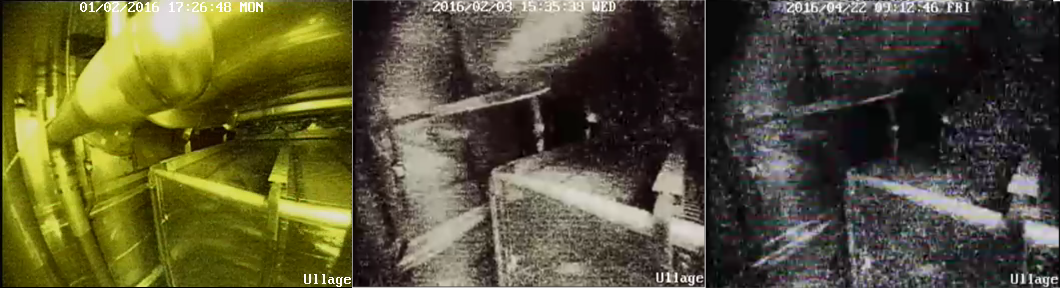
\includegraphics[width=\textwidth]{Cam1degradation2}
    \caption{The degradation in signal quality of the camera focused on the ullage.}
  \end{subfigure}
  \begin{subfigure}{0.95\textwidth}
    \centering
    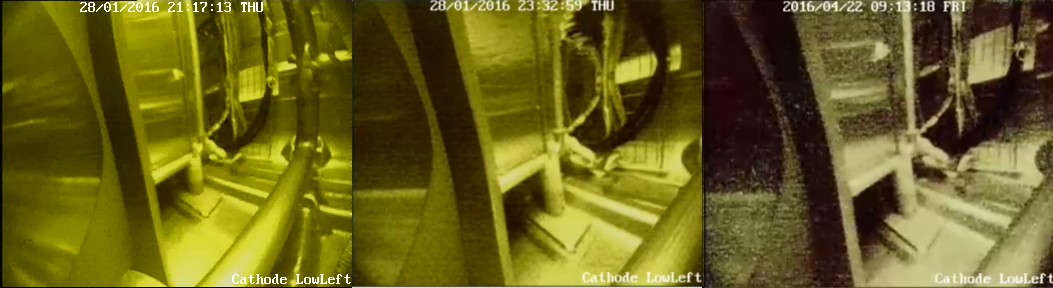
\includegraphics[width=\textwidth]{Cam4degradation2}
    \caption{The degradation in signal quality of the camera focused on the lower left corner of the cathode.}
  \end{subfigure}
  \caption[The signal degradation over time for two cameras in the 35 ton camera system]
          {The signal degradation over time for two cameras in the 35 ton camera system. Top shows the signal degradation observed for the camera focused on the ullage. Bottom shows the signal degradation for the camera focused on the lower left corner of the cathode. For both cameras, left shows the field-of-view prior to cool down, centre shows the field-of-view immediately after cool down, and right shows the field-view after 10 weeks of operation. These are full colour images, as recorded by the DVR, and so no post-processing has been performed on the images.}  
  \label{fig:CamSigDeg}
\end{figure}

From Figure~\ref{fig:CamSigDeg}, it can be seen over the course of the run, the fields-of-view for both cameras became more pixelated, and that there was an increase in the number of pixels which were either saturated, or dead. The large number of saturated pixels was particularly evident when the cryostat was not illuminated, and meant that the region which could be used to trigger on HV breakdowns was severely limited for some cameras. As shown, this degradation was highly camera specific, with the resolution of the ullage camera deteriorating severely, whilst the camera focusing on the lower left corner of the cathode is relatively unchanged over the course of the run. A striking difference between the left-most images, and the central and right-most images, in Figure~\ref{fig:CamSigDeg}, is the loss of colour in the images which are produced. This is attributed to a partial failure of the on-board encoding circuits, which resulted in the colour signal streams not being functional when exposed to cryogenic temperatures. This loss of colour was seen as soon as the cameras were exposed to cryogenic temperatures, and was also observed in the initial tests performed in Sheffield. \\

It is important to note that the cameras were able to operate safely within their modules, and did not impinge on any other systems in the cryostat. They were also found to be able to be power cycled after large periods of time in the cold, including after not being operational for a large period of time. One such period, which lasted for 9 days, was when the cameras were powered off whilst extensive noise hunting was performed. Upon being power cycled, all 8 cameras were immediately brought back online, without the need for the inbuilt heaters. \\

During normal operation of the 35 ton system, the high voltage operated stably at 60 kV, and so no breakdowns were observed. However, after the cathode was raised to 135 kV in low-purity argon, three of four breakdowns were detected by the camera system, and data was written to disk as expected. Unfortunately, the cameras were not able to pinpoint the exact locations of the breakdowns, and so their effectiveness at discerning the locations of HV breakdowns is still largely untested. Despite this, however, the cameras proved to be a very valuable monitoring tool in the 35 ton cryostat, and there has been interest in including analogous systems in future LArTPCs, such as SBND~\citep{SBNProposal}. \\
